%%%%%%%%%%%%%%%%%%%%%%%%%%%%%%%%%%%%%%%%%
% Beamer Presentation
% LaTeX Template
% Version 1.0 (10/11/12)
%
% This template has been downloaded from:
% http://www.LaTeXTemplates.com
%
% License:
% CC BY-NC-SA 3.0 (http://creativecommons.org/licenses/by-nc-sa/3.0/)
%
%%%%%%%%%%%%%%%%%%%%%%%%%%%%%%%%%%%%%%%%%

%----------------------------------------------------------------------------------------
%	PACKAGES AND THEMES
%----------------------------------------------------------------------------------------

\documentclass{beamer}

\mode<presentation> {

% The Beamer class comes with a number of default slide themes
% which change the colors and layouts of slides. Below this is a list
% of all the themes, uncomment each in turn to see what they look like.

%\usetheme{default}
%\usetheme{AnnArbor}
%\usetheme{Antibes}
%\usetheme{Bergen}
%\usetheme{Berkeley}
%\usetheme{Berlin}
%\usetheme{Boadilla}
%\usetheme{CambridgeUS}
%\usetheme{Copenhagen}
%\usetheme{Darmstadt}
%\usetheme{Dresden}
%\usetheme{Frankfurt}
%\usetheme{Goettingen}
%\usetheme{Hannover}
%\usetheme{Ilmenau}
%\usetheme{JuanLesPins}
%\usetheme{Luebeck}
\usetheme{Madrid}
%\usetheme{Malmoe}
%\usetheme{Marburg}
%\usetheme{Montpellier}
%\usetheme{PaloAlto}
%\usetheme{Pittsburgh}
%\usetheme{Rochester}
%\usetheme{Singapore}
%\usetheme{Szeged}
%\usetheme{Warsaw}

% As well as themes, the Beamer class has a number of color themes
% for any slide theme. Uncomment each of these in turn to see how it
% changes the colors of your current slide theme.

%\usecolortheme{albatross}
%\usecolortheme{beaver}
%\usecolortheme{beetle}
%\usecolortheme{crane}
%\usecolortheme{dolphin}
%\usecolortheme{dove}
%\usecolortheme{fly}
%\usecolortheme{lily}
%\usecolortheme{orchid}
%\usecolortheme{rose}
%\usecolortheme{seagull}
%\usecolortheme{seahorse}
%\usecolortheme{whale}
%\usecolortheme{wolverine}

%\setbeamertemplate{footline} % To remove the footer line in all slides uncomment this line
%\setbeamertemplate{footline}[page number] % To replace the footer line in all slides with a simple slide count uncomment this line

%\setbeamertemplate{navigation symbols}{} % To remove the navigation symbols from the bottom of all slides uncomment this line
}

\usepackage{graphicx} % Allows including images
\usepackage{booktabs} % Allows the use of \toprule, \midrule and \bottomrule in tables
\usepackage{amsmath}
\usepackage{enumitem}


%----------------------------------------------------------------------------------------
%	TITLE PAGE
%----------------------------------------------------------------------------------------

\title[Nonlinear Market Impact]{A Minimal Model for Nonlinear Market Impact} 

\author{ShengQuan Zhou, Zhongkai He} % Your name
\institute[Baruch] 
{
Baruch MFE \\ % Your institution for the title page
}

\date{\today} % Date, can be changed to a custom date
\titlegraphic{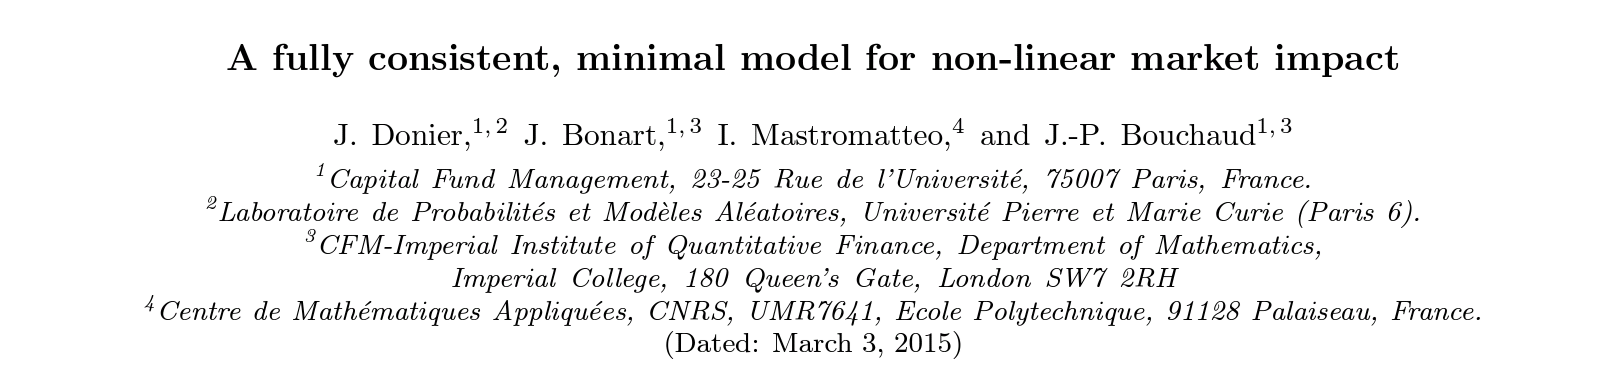
\includegraphics[width=\textwidth,height=.3\textheight]{paper}}

\begin{document}

\begin{frame}
\titlepage % Print the title page as the first slide
\end{frame}



\begin{frame}
\frametitle{A Reaction-Diffusion Model of Latent Order Book}
{
\footnotesize{
\begin{columns}
\begin{column}{0.4\textwidth}
   \underline{Two pivotal ideas}
   \begin{itemize}
       \item Latent order book
       \item Reaction-Diffusion model
   \end{itemize}
   \underline{Order Book Dynamics $(x:\text{price})$}
   \begin{itemize}
       \item Buy volume density $\rho_B(x,t)$
       \item Sell volume density $\rho_A(x,t)$
   \end{itemize}
   \underline{Transaction Price $p_t$}
   $$
   \boxed{
       \rho_A(p_t, t) = \rho_B(p_t, t) 
       }  
   $$
\end{column}
\begin{column}{0.6\textwidth}  %%<--- here
    \begin{center}
     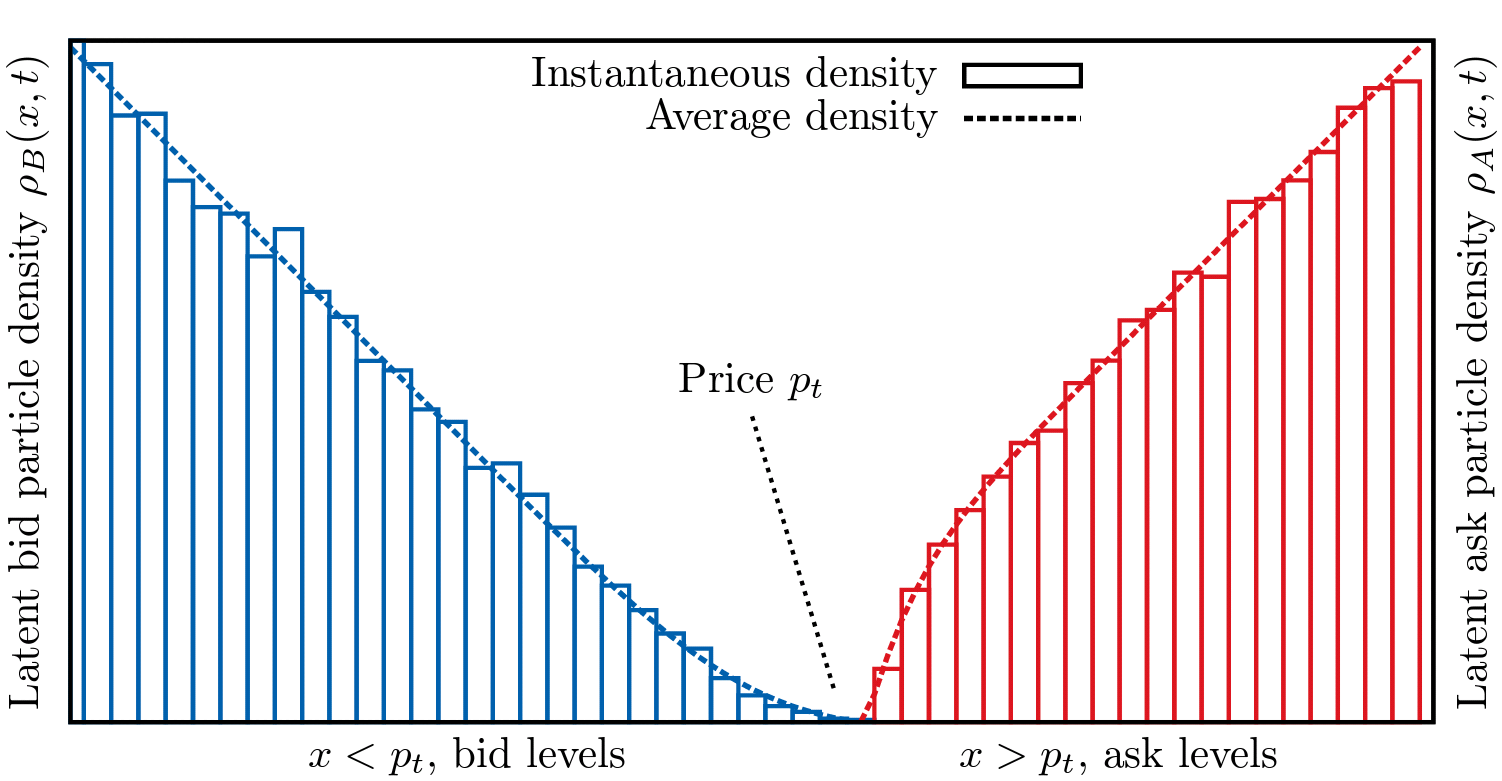
\includegraphics[width=\textwidth,height=.5\textheight]{llob}
     \end{center}
\end{column}
\end{columns}

\begin{align*}
\frac{\partial \rho_B(x,t)}{\partial t} &= -V_t \frac{\partial \rho_B(x,t)}{\partial x}
+ D  \frac{\partial^2 \rho_B(x,t)}{\partial x^2} -\nu \rho_B(x,t) +\lambda \Theta(p_t -x) - \kappa R_{AB}(x,t)\\
\frac{\partial \rho_A(x,t)}{\partial t} &= \underbrace{-V_t \frac{\partial \rho_A(x,t)}{\partial x}
+ D  \frac{\partial^2 \rho_A(x,t)}{\partial x^2}}_{\begin{subarray}{l}\text{\text{Drift-Diffusion: price reassessments;}}\\
    V_t\sim\text{\text{white noise, uninformed meta-orders}}\end{subarray} } -\underbrace{\nu \rho_A(x,t)}_{\text{Cancellation}} +\underbrace{\lambda \Theta(x-p_t)}_{\text{Deposition}} - \underbrace{\kappa R_{AB}(x,t)}_{\text{Reaction: trades}}
\end{align*}

}
}
\end{frame}


\begin{frame}
\frametitle{Price Dynamics within a Locally Linear Order Book}
{
\footnotesize{
Define $\hat{p}_t \triangleq \int_0^t V_s ds$, $y\triangleq x-\hat{p}_t$, the net order density $\phi(x,t)\triangleq \rho_B(x,t)-\rho_A(x,t)$
\begin{columns}
\begin{column}{0.7\textwidth}
   $$
   \quad\quad\quad\quad\quad\frac{\partial \phi(y,t)}{\partial t} = D\frac{\partial^2 \phi(y,t)}{\partial y^2} -\nu \phi(y,t) + \lambda
   \text{sign}(p_t - \hat{p}_t - y)
   $$
\end{column}
\begin{column}{0.3\textwidth}  %%<--- here
     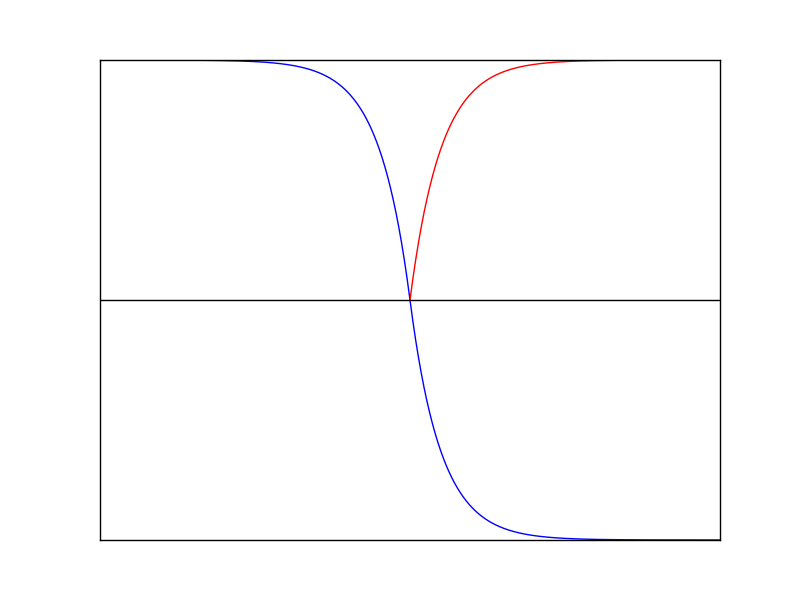
\includegraphics[width=\textwidth,height=.15\textheight]{phist}
\end{column}
\end{columns}
Zoom into the \textit{\color{blue}{universal linear regime}}
$\nu\rightarrow 0$, $\lambda\rightarrow 0$, $J \triangleq D\left|\partial_y \phi_{\text{s.t.}} \right|_{y=0} = \lambda\sqrt{D/\nu}$ fixed:
\begin{columns}
\begin{column}{0.7\textwidth}
$$
\quad\quad\quad\quad\quad\phi_{\text{s.t.}} = -\mathcal{L} y,
$$
\end{column}
\begin{column}{0.3\textwidth}  %%<--- here
     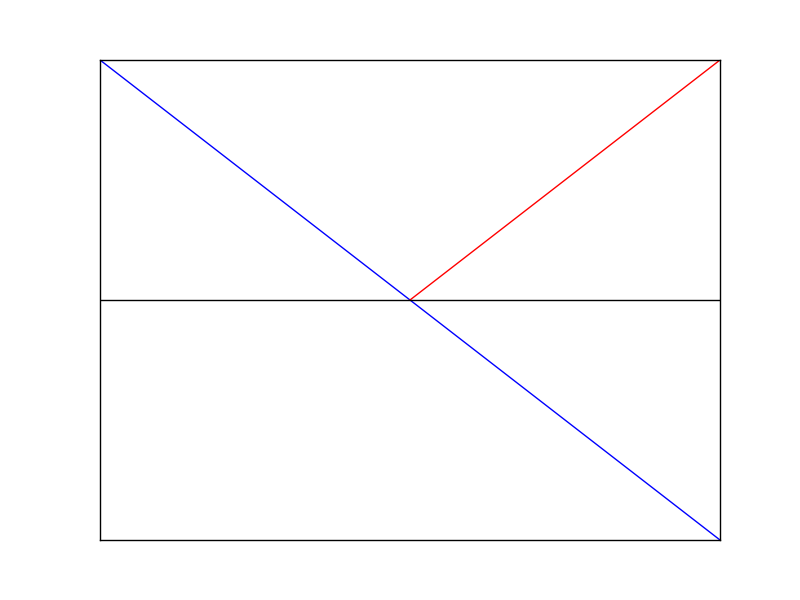
\includegraphics[width=\textwidth,height=.1\textheight]{linear}
\end{column}
\end{columns}

where $\mathcal{L}\triangleq J/D$ is the \textit{\color{blue}{latent liquidity}} of the market. Add \underline{meta-order}
to the system:
$$
\begin{cases}
\frac{\partial \phi(y,t)}{\partial t} = D\frac{\partial^2 \phi(y,t)}{\partial y^2}  + m_t \delta(y-y_t)\\
\partial_y \phi(y\rightarrow \pm\infty, t) = -\mathcal{L}
\end{cases}
\Rightarrow \phi(y,t) = -\mathcal{L}y + \int_0^t \frac{ds \, m_s}{\sqrt{4\pi(t-s)}} e^{-\frac{(y-y_s)^2}{4D(t-s)}}
$$
where $m_t$ is the signed trading intensity at time $t$. \underline{Transaction price} $\phi(y_s, s)\equiv 0$
$$
\boxed{
y_t = \frac{1}{\mathcal{L}}\int_0^t \frac{ds \, m_s}{\sqrt{4\pi(t-s)}} e^{-\frac{(y_t-y_s)^2}{4D(t-s)}}
}
$$ 
This is the \underline{central equation} of the paper: a self-consistent integral equation for $t>0$.
}
}
\end{frame}

\begin{frame}
\frametitle{Impact of Meta-Order and Impact Decay}
{
\footnotesize{
For a meta-order of size $Q$ executed at \underline{constant rate}
$
m_t = \begin{cases}
 m_0 = Q/T, \, &t\in[0,T],\\
 0, \, &t>T.
\end{cases}
$

\underline{Market Impact} $\mathcal{I}(Q,t) \triangleq \underbrace{\langle \epsilon\cdot(p_{t+T} - p_t) |Q\rangle}_{\text{Average over order signs } \epsilon}
=  \langle \epsilon\cdot(y_{t+T} - y_t) |Q\rangle \underbrace{\textcolor{gray}{+ \langle \epsilon\cdot(\hat{p}_{t+T} - \hat{p}_t) |Q\rangle}}_{\text{=0, uninformed meta-order}}$.

Solving the \underline{self-consistency} equation for $y_t$ yields the \textit{\color{blue}{impact profile}}:
\begin{columns}
\begin{column}{0.55\textwidth}
\begin{align*}
\frac{\mathcal{I}(Q,t)}{\mathcal{I}(Q)} = 
\begin{cases}
\sqrt{\frac{t}{T}}, \, &t\in[0,T],\\
\underbrace{\sqrt{\frac{t}{T}} - \sqrt{\frac{t-T}{T}}}_{\text{power-law decay as } t\rightarrow\infty}, \,  &t>T,
\end{cases}
\end{align*}
where the peak market impact gives precisely the celebrated \textit{\color{blue}{square-root impact law}}:
$$
\mathcal{I}(Q) = \mathcal{I}(Q,T) \approx \begin{cases}
\sqrt{\frac{m_0}{\pi J}}\times\sqrt{\frac{Q}{\mathcal{L}}}, \, & m_0 \ll J,\\
\sqrt{2}\times \sqrt{\frac{Q}{\mathcal{L}}}, \, & m_0 \gg J.
\end{cases}
$$
\end{column}
\begin{column}{0.45\textwidth}  %%<--- here
    \begin{center}
     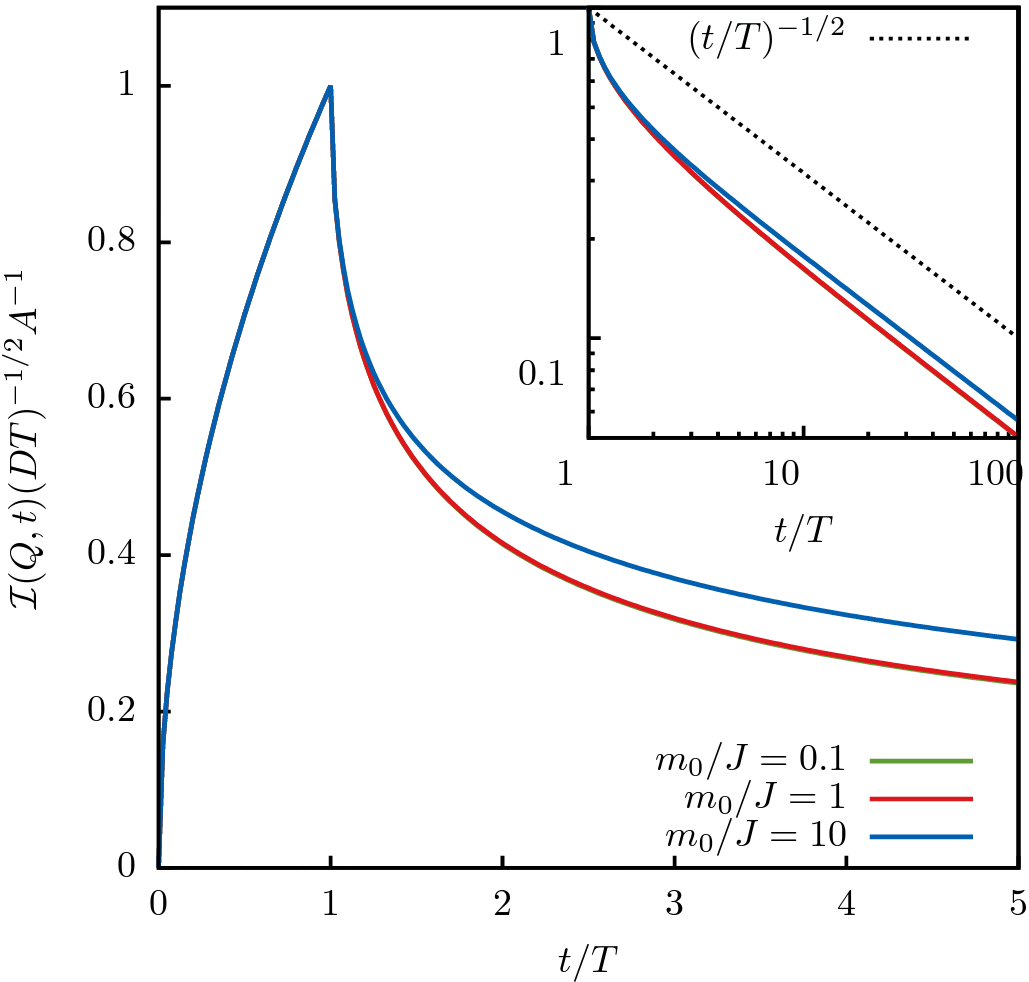
\includegraphics[width=\textwidth,height=.5\textheight]{impact}
     \end{center}
\end{column}
\end{columns}

}
}
\end{frame}

\begin{frame}
\frametitle{Reversions, Informational Impact \& No Price Manipulation}
{
\footnotesize{

$\square$ For a meta-order of size $Q$ \underline{reverted} after $T$,
$
m_t = \begin{cases}
 m_0 = Q/T, \, &t\in[0,T],\\
 -m_0 = -Q/T, \, &t\in (T,2T].
\end{cases}
$

$\square$ \underline{Informative order flow} $m_t$ correlated with order book drift $V_{t'>t}$: \textit{\color{blue}{permanent impact}}.

\begin{columns}
\begin{column}{0.05\textwidth}  %%<--- here
\end{column}
%\begin{column}{0.33\textwidth}
%    \begin{center}
%     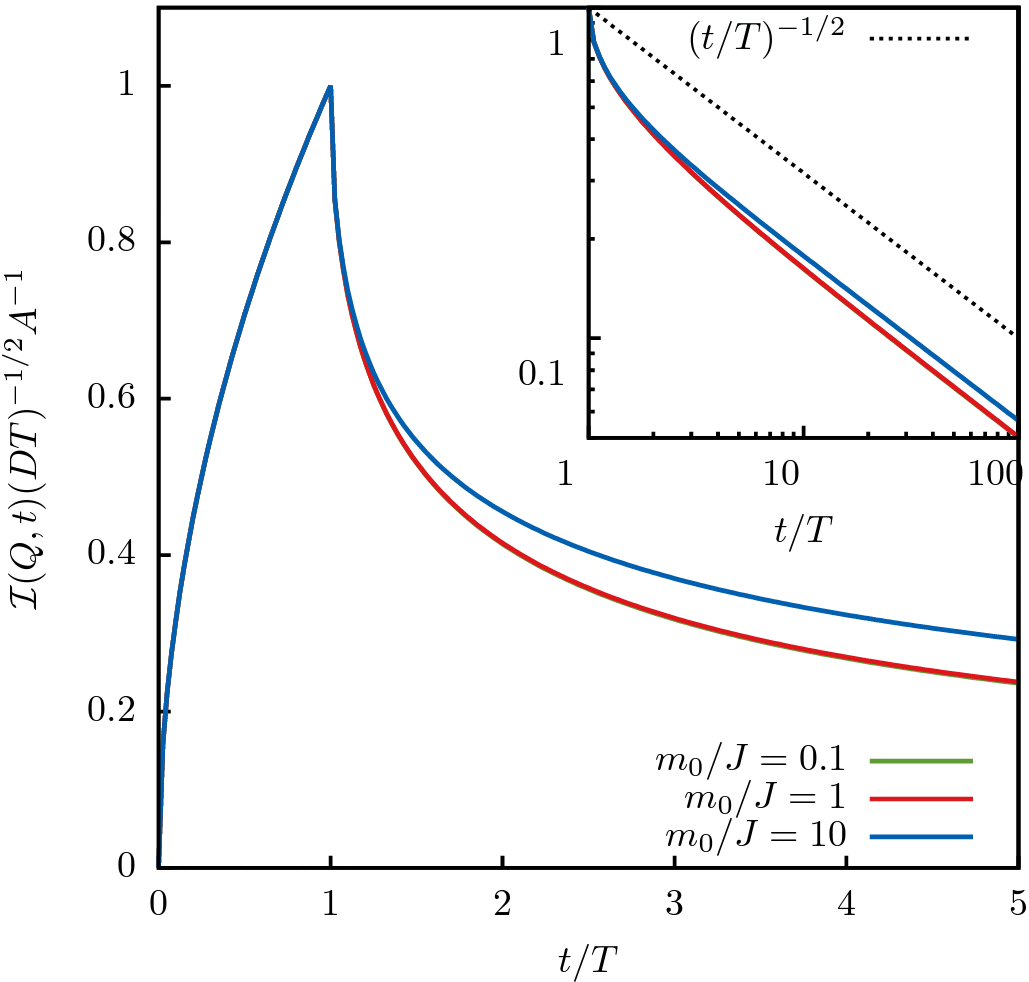
\includegraphics[width=0.89\textwidth,height=.3\textheight]{impact}
%    \end{center}
%\end{column}
\begin{column}{0.45\textwidth}
    \begin{center}
     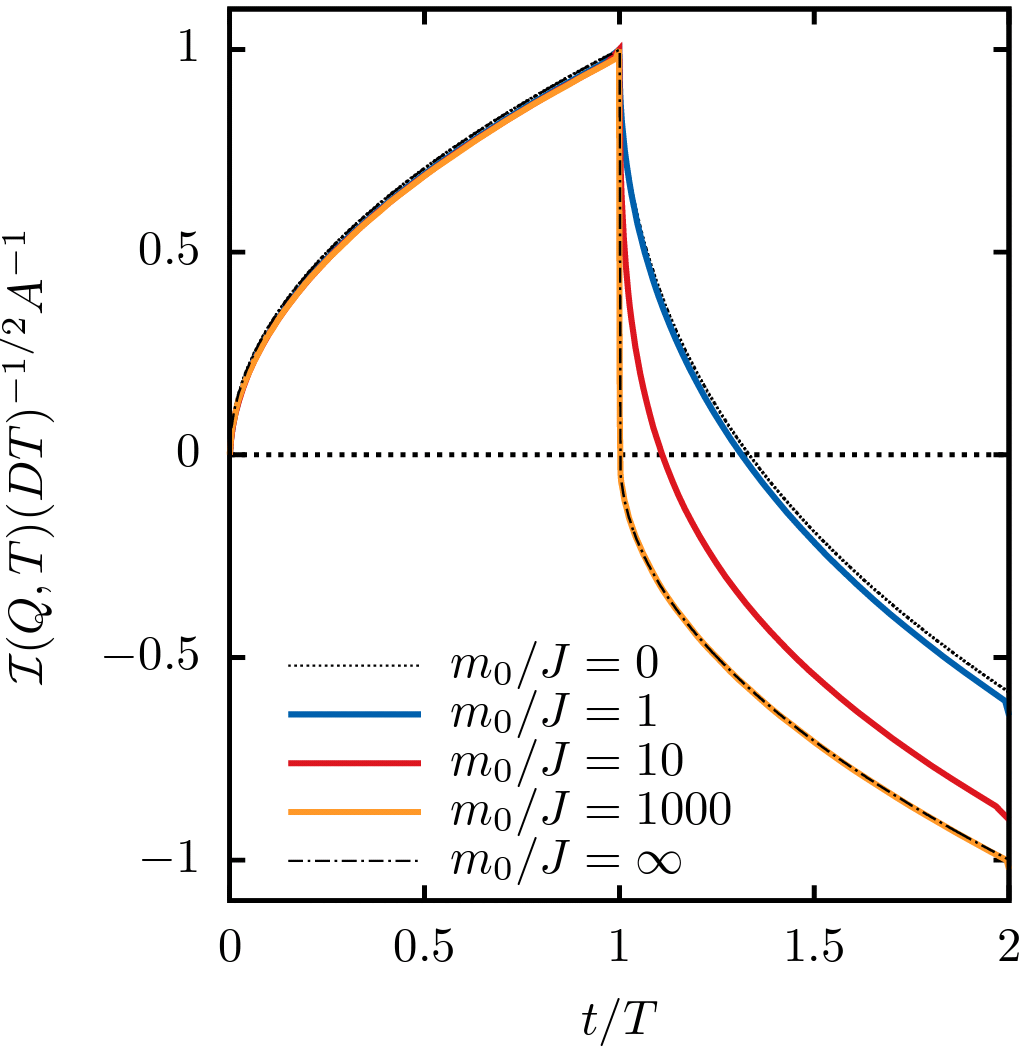
\includegraphics[width=0.93\textwidth,height=.35\textheight]{reversion}
    \end{center}
\end{column}
\begin{column}{0.45\textwidth}  %%<--- here
    \begin{center}
     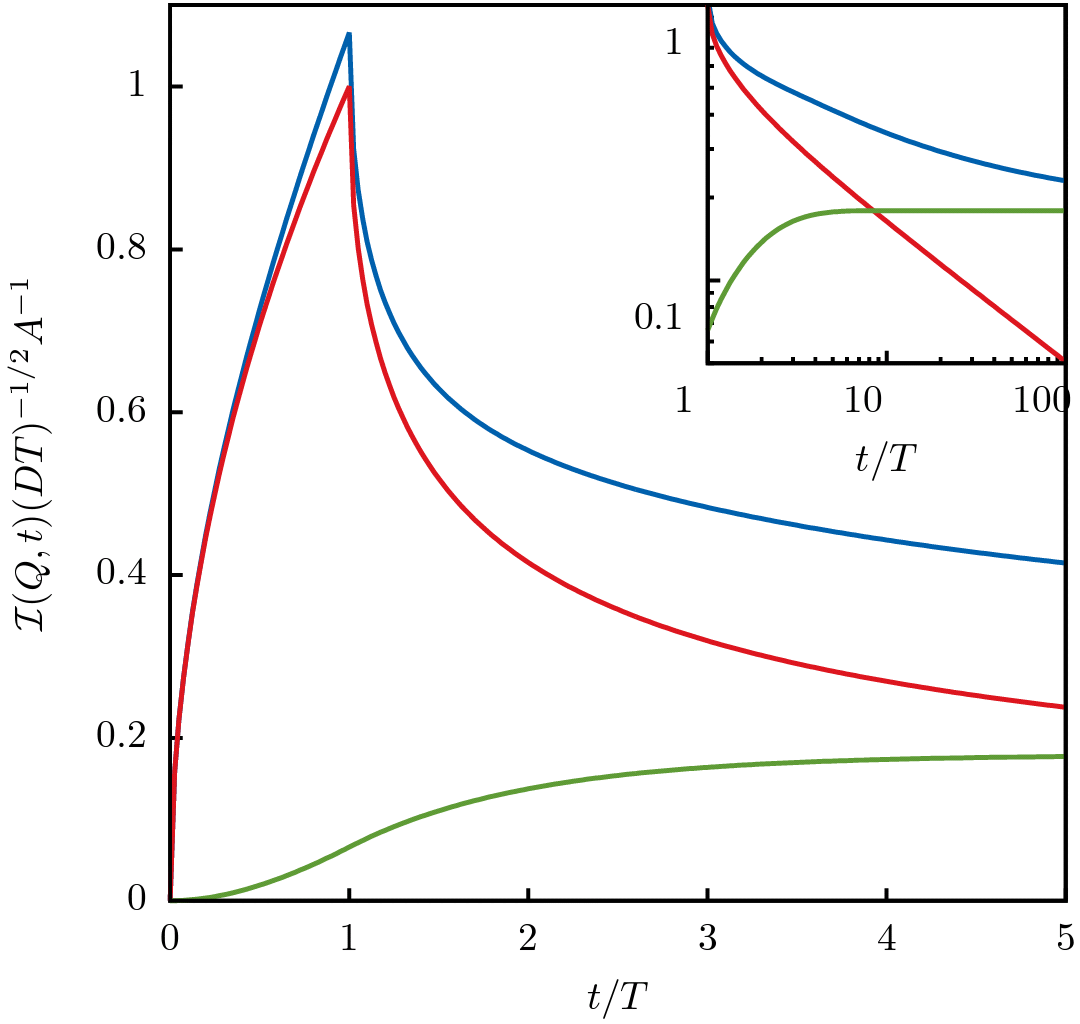
\includegraphics[width=0.85\textwidth,height=.35\textheight]{permanent}
    \end{center}
\end{column}
\begin{column}{0.5\textwidth}  %%<--- here
\end{column}
\end{columns}


$\square$ Average cost of a \underline{closed price trajectory}: $\int_0^T ds\,m_s = 0$. 
$$
\mathcal{C} = \int_0^T ds\, m_s y_s = \frac{1}{2} \int_0^T \int_0^T ds ds'\,  M(s,s') m_s m_{s'}
$$
where
$
M(s,s') = \frac{1}{\mathcal{L}\sqrt{4\pi|s-s'|}}e^{-\frac{(y_s-y_{s'})^2}{4D|s-s'|}}
$
is a semi-positive definite kernel $\Rightarrow \mathcal{C}\ge 0$ for any execution schedule, i.e. price
manipulation is impossible within the model of Locally Linear Order Book (LLOB).
\newline
}

%\newline
%\underline{\textbf{Possible Extensions and Open Problems}}

%\begin{itemize}[noitemsep]
%\item $\square$ Relax the approximation made in limit of
%    \begin{itemize}[noitemsep]
%        \item (1) slow latent order books $\nu T \ll 1$;
%        \item (2) large liquidity, i.e., meta-order only probes the linear region of order book.
%    \end{itemize}
%\item $\square$ Corrections to the LLOB induced by fluctuations.
%\item $\square$ Introduce random fluctuations in the interacting meta-order flows.
%\item $\square$ Cancellation rate $\nu$ is expected to increase with the intensity of meta-orders.
%\item $\square$ Deposition rate $\lambda$ is expected to increase with the distance $|x-p_t|$.
%\item $\square$ Drift term $V_t$ could be non-Gaussian.
%\end{itemize}
}

\end{frame}

\end{document} 